% Provenance (never printed): see sources/outline_sources.md (Year 1: vertical structure of
% the atmosphere, lapse rates, potential temperature and static stability; the layered
% ocean, the equation of state of seawater, T-S diagrams and water masses). Exercise and
% problem values in the Book 3 scratch calculator calc/ch26.py; figures from
% figdata/bachelor-1/atmosphere_profile.py (U.S. Standard Atmosphere 1976) and
% seawater_eos.py (EOS-80 and the UNESCO 44 algorithms; WOA23 columns, datasets
% bachelor-1-woa23-* and Book 2's grade-10-woa23-arctic-*).
% Physics owns the hydrostatic relation, the isothermal atmosphere and its scale height,
% the first law, Laplace's relation and Archimedes' thrust (recalled). Book 1 (g8) gave
% the layers and the environmental lapse rate of 6.5 K/km; Book 2 (g10) the dry adiabatic
% rate admitted, stable and unstable air, the mixed layer, thermocline, halocline and
% pycnocline: re-founded here with derivations. The moist adiabat is the Year 2 volume's.
\chapter{Estructura de la atmósfera y del océano}\label{ch:b1:fluid-envelopes-structure}

Dos veces al día, en estaciones meteorológicas de todo el mundo, se suelta un globo que lleva una radiosonda, un pequeño instrumento que transmite por radio la presión, la temperatura y la humedad del aire a medida que asciende; sube a unos \qty{300}{m} por minuto y puede pasar de \qty{35}{km} antes de que el globo reviente. Muy lejos en el mar, un buque de investigación baja al abismo, por un cable, un bastidor de instrumentos y botellas de agua, y mide en todo el trayecto la conductividad, la temperatura y la profundidad. Los dos perfiles, uno del aire y otro del agua, son la materia prima de este capítulo. Ambas envolturas están estratificadas, y en ambas la estratificación la fija la densidad: el fluido ligero encima del pesado. Lo que hace que una capa sea ligera o pesada es menos obvio de lo que parece. El aire más frío que el aire de debajo puede ser, aun así, el más ligero; el agua más cálida que la de encima puede ser, aun así, la más pesada. El capítulo construye las dos herramientas que ordenan esto: la \omterm{def:b1:fluid-envelopes-structure:potential-temperature}{temperatura potencial} y la \omterm{def:b1:fluid-envelopes-structure:eos}{ecuación de estado del agua de mar}.
% ledger: nws:radiosonde, nws:radiosonde-def, commons:ctd-rosette

\begin{omfigure}
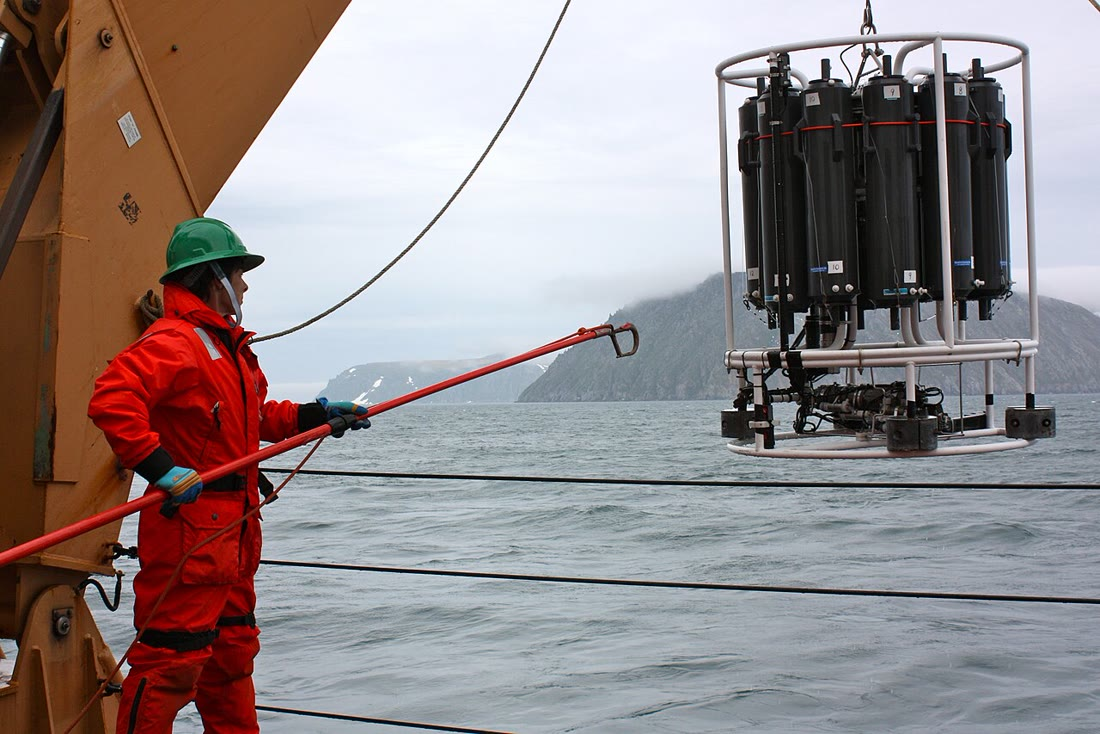
\includegraphics[width=0.62\linewidth]{images/book3/b1-ctd-rosette.jpg}

{\small Un CTD y una roseta subidos a bordo en el estrecho de Bering en junio de 2011. Las botellas grises alrededor del bastidor se cierran a profundidades escogidas durante la subida para muestrear el agua; los instrumentos de la parte inferior del bastidor miden de forma continua la conductividad (de la que se calcula la salinidad), la temperatura y la profundidad (en realidad, la presión) mientras el bastidor desciende. (NASA Goddard Space Flight Center, dominio público, vía Wikimedia Commons.)}
\label{fig:b1:fluid-envelopes-structure:ctd}
\end{omfigure}
% ledger: commons:ctd-rosette, unesco44:atg-theta

\begin{recall}
Los libros de física dan la relación hidrostática, $\mathrm dp/\mathrm dz =
-\rho g$, para un fluido en reposo; para un gas ideal de masa molar $M$, $p = \rho R
T/M$, y en una atmósfera isoterma la presión decrece como $e^{-z/H}$ con la
altura de escala $H = RT/(Mg)$. Establecen el primer principio para un sistema cerrado y, para un gas ideal, la relación de Laplace a lo largo de una transformación adiabática reversible,
$pV^{\gamma} = $ constante, con $\gamma = c_p/c_v$ y $c_p - c_v
= R/M$ por unidad de masa. Un cuerpo sumergido en un fluido recibe un empuje hacia arriba igual al peso del fluido que desplaza (Arquímedes). El libro 1 nombró las capas de la atmósfera y el \omterm{def:b1:fluid-envelopes-structure:lapse-rate}{gradiente ambiental} de la \omterm{def:b1:fluid-envelopes-structure:standard-atmosphere}{atmósfera estándar}, \qty{6.5}{\celsius} por kilómetro en la troposfera; el libro 2 admitió el \omterm{def:b1:fluid-envelopes-structure:lapse-rate}{gradiente adiabático seco}, \qty{9.8}{\celsius} por kilómetro, llamó estable o inestable al aire según el destino de una porción empujada hacia arriba, y describió la \omterm{def:b1:fluid-envelopes-structure:ocean-layers}{capa de mezcla}, la \omterm{def:b1:fluid-envelopes-structure:ocean-layers}{termoclina}, la \omterm{def:b1:fluid-envelopes-structure:ocean-layers}{haloclina} y la \omterm{def:b1:fluid-envelopes-structure:ocean-layers}{picnoclina} del océano. La salinidad del agua de mar es cercana a 35 gramos de sales disueltas por kilogramo.
% ledger: ussa76:layers, nws:dalr, nos:salinity
\end{recall}

\section{Estructura vertical de la atmósfera}\label{sec:b1:fluid-envelopes-structure:atmosphere}

No hay dos sondeos reales iguales. Para compararlos, se fija por convención un perfil de referencia.

\begin{definition}[Atmósfera estándar]\label{def:b1:fluid-envelopes-structure:standard-atmosphere}
Una \emph{atmósfera estándar}\index{atmósfera estándar} es un perfil de
temperatura, presión y densidad frente a la altura, fijado por convención: aire seco de masa molar constante, un gas ideal en equilibrio hidrostático, con valores dados al nivel del mar y una temperatura que varía linealmente con la altura en capas sucesivas. La atmósfera estándar de 1976 toma \qty{288.15}{K} y
\qty{101325}{Pa} al nivel del mar, $M_0 = \qty{28.9644}{kg.kmol^{-1}}$,
$R^* = \qty{8314.32}{J.kmol^{-1}.K^{-1}}$ y $g_0 = \qty{9.80665}{m.s^{-2}}$.
\end{definition}
% ledger: ussa76:sea-level

Por debajo de \qty{47}{km}, la \omterm{def:b1:fluid-envelopes-structure:standard-atmosphere}{atmósfera estándar} de 1976 tiene cuatro capas
(\cref{tab:b1:fluid-envelopes-structure:layers}). La más baja, la troposfera, se enfría a \qty{6.5}{K} por kilómetro; desde su techo, la tropopausa, la temperatura se mantiene en \qty{216.65}{K} durante nueve kilómetros, y luego sube. Las alturas de la estándar son alturas geopotenciales, las alturas que daría una gravedad constante $g_0$ con la misma energía potencial; por debajo de \qty{32}{km} difieren de las alturas geométricas en menos de un \qty{0.6}{\percent}
(\qty{11}{km} de la estándar caen a \qty{11.02}{km}).
% ledger: ussa76:layers, ussa76:sea-level

\begin{table}[ht]
\centering
\small
\renewcommand{\arraystretch}{1.2}
\begin{tabular}{|l|c|c|c|c|}
\hline
Capa & Base (km) & $\mathrm dT/\mathrm dz$ (K/km) & $T$ en la base (K) & $p$ en la base (hPa) \\
\hline
1 (troposfera) & 0 & $-6.5$ & 288.15 & 1013.25 \\
2 (estratosfera) & 11 & 0.0 & 216.65 & 226.32 \\
3 (estratosfera) & 20 & $+1.0$ & 216.65 & 54.75 \\
4 (estratosfera) & 32 & $+2.8$ & 228.65 & 8.68 \\
\hline
\end{tabular}
\caption{Las cuatro capas más bajas de la \omterm{def:b1:fluid-envelopes-structure:standard-atmosphere}{atmósfera estándar} de 1976. Los gradientes y los valores al nivel del mar son valores que definen la estándar; las temperaturas y presiones en las bases se calculan a partir de ellos con \cref{prop:b1:fluid-envelopes-structure:layer-pressure}.}
\label{tab:b1:fluid-envelopes-structure:layers}
\end{table}
% ledger: ussa76:layers, ussa76:sea-level (bases computed in figdata/bachelor-1/atmosphere_profile.py)

En cada capa la temperatura es una función lineal de la altura, así que la relación hidrostática puede integrarse en forma cerrada.

\begin{proposition}[Presión en una capa de gradiente constante]\label{prop:b1:fluid-envelopes-structure:layer-pressure}
En una capa de aire seco donde $T = T_b - L\,(z - z_b)$ con un $L \neq 0$ constante, la
presión es
\[
  p = p_b \left(\frac{T}{T_b}\right)^{gM/(RL)},
\]
donde $T_b$ y $p_b$ son los valores en la base $z_b$. Cuando $L = 0$ la presión decrece exponencialmente con la altura de escala $H = RT_b/(Mg)$.
\end{proposition}

\begin{proof}
La relación hidrostática y el gas ideal dan $\mathrm dp/p = -(gM/R)\,\mathrm
dz/T$. Como $\mathrm dT = -L\,\mathrm dz$, esto es $\mathrm dp/p =
(gM/(RL))\,\mathrm dT/T$, que integra a $\ln(p/p_b) = (gM/(RL))
\ln(T/T_b)$. Para $L = 0$, $T = T_b$ y $\ln(p/p_b) = -(z - z_b)/H$: la atmósfera isoterma de los libros de física.
\end{proof}

En la troposfera de la estándar, $gM/(RL) = 9.80665 \times 28.9644 /
(8314.32 \times 0.0065) = 5.256$, y a \qty{11}{km}, $T = 216.65$~K:
$p = \num{101325} \times (216.65/288.15)^{5.256} = \qty{22632}{Pa}$, algo
menos de una cuarta parte del valor al nivel del mar. En la capa isoterma de encima, $H =
8314.32 \times 216.65/(28.9644 \times 9.80665) = \qty{6.34}{km}$, y nueve
kilómetros más arriba la presión ha caído en un factor adicional $e^{9/6.34} =
4.13$, hasta \qty{5475}{Pa}. Como la presión a un nivel es el peso, por unidad de
área, del aire que tiene encima, la mitad de la masa de la \omterm{def:b1:fluid-envelopes-structure:standard-atmosphere}{atmósfera estándar} queda por debajo de \qty{5.5}{km} y nueve décimas partes por debajo de \qty{16}{km}.
% ledger: ussa76:sea-level, ussa76:layers (values computed in figdata/bachelor-1/atmosphere_profile.py)

\section{Gradientes térmicos y temperatura potencial}\label{sec:b1:fluid-envelopes-structure:lapse}

\begin{definition}[Gradientes térmicos ambiental y adiabático seco]\label{def:b1:fluid-envelopes-structure:lapse-rate}
El \emph{gradiente ambiental}\index{gradiente ambiental} es $\Gamma =
-\mathrm dT/\mathrm dz$, la velocidad a la que decrece con la altura la temperatura del aire en reposo, tal como la mide un sondeo. El \emph{gradiente adiabático
seco}\index{gradiente adiabático seco} $\Gamma_d$ es la velocidad a la que decrece la temperatura de una porción de aire no saturado a medida que se eleva.
\end{definition}
% ledger: nws:dalr

Una tasa de variación es positiva cuando la temperatura disminuye con la altura. Las dos tasas son de naturaleza distinta: la primera describe el estado de la atmósfera en un instante; la segunda, la transformación de una porción de aire que se mueve.

\begin{definition}[Partícula de aire]\label{def:b1:fluid-envelopes-structure:parcel}
Una \emph{partícula de aire}\index{partícula de aire} es un volumen de aire que se sigue en su movimiento, lo bastante pequeño para tener una sola temperatura y presión y no perturbar el aire de alrededor, y lo bastante grande para conservar su identidad: no intercambia masa y, durante un desplazamiento rápido, tampoco calor con su entorno, y su presión es en todo momento la del aire que la rodea.
\end{definition}

La partícula es una idealización, como el sistema cerrado de la termodinámica: los resultados siguientes valen para el aire real en la medida en que una porción en movimiento intercambia poco calor y poca masa con su entorno.

\begin{theorem}[El gradiente adiabático seco]\label{thm:b1:fluid-envelopes-structure:dry-adiabatic}
Una \omterm{def:b1:fluid-envelopes-structure:parcel}{partícula de aire} seco, elevada adiabática y reversiblemente a través de aire en reposo de temperatura casi igual, se enfría a la velocidad
\[
  \Gamma_d = \frac{g}{c_p},
\]
donde $c_p$ es el calor específico del aire a presión constante. Con $c_p =
\qty{1004.7}{J.kg^{-1}.K^{-1}}$, $\Gamma_d = \qty{9.76}{K.km^{-1}}$.
\end{theorem}

\begin{proof}
Para un kilogramo de la partícula, de temperatura $T_p$ y densidad $\rho_p$, la primera ley de una transformación reversible sin intercambio de calor, escrita con la entalpía, es $c_p\,\mathrm dT_p - \mathrm dp/\rho_p = 0$. La presión de la partícula es la del aire circundante, que es hidrostática: $\mathrm dp = -\rho_e
g\,\mathrm dz$, con $\rho_e$ la densidad del aire circundante. Por tanto
\[
  \frac{\mathrm dT_p}{\mathrm dz} = -\frac{g}{c_p}\,\frac{\rho_e}{\rho_p}
  = -\frac{g}{c_p}\,\frac{T_p}{T_e},
\]
pues a la misma presión las densidades de dos gases ideales de la misma masa molar
están en razón inversa de sus temperaturas. Cuando la partícula está casi a la temperatura de su entorno, $T_p/T_e \approx 1$ y $-\mathrm dT_p/\mathrm dz
= g/c_p$. Para el aire seco, un gas diatómico ideal, $\gamma = 1.4$, así que $c_p =
\gamma/(\gamma - 1) \times R/M = 3.5 \times 8314.32/28.9644 =
\qty{1004.7}{J.kg^{-1}.K^{-1}}$, y $\Gamma_d = 9.80665/1004.7 =
\qty{0.00976}{K.m^{-1}}$.
\end{proof}
% ledger: nasa:grc-gamma, ussa76:sea-level, nws:dalr

Una partícula \qty{10}{K} más cálida que su entorno, cerca de \qty{280}{K}, se enfría a
$\Gamma_d \times 290/280$, un \qty{3.6}{\percent} más deprisa; la corrección se
omite en lo que sigue. La velocidad no depende de la presión ni de la temperatura de la partícula, y una partícula que desciende se calienta a la misma velocidad, como siguió el libro 2 el aire sobre una montaña.

Integrar la misma ecuación sin el paso hidrostático da una magnitud que
la partícula lleva consigo.

\begin{proposition}[Temperatura potencial]\label{prop:b1:fluid-envelopes-structure:theta}
A lo largo de una transformación adiabática reversible del aire seco,
\[
  \theta = T\left(\frac{p_0}{p}\right)^{\kappa},\qquad \kappa = \frac{R}{Mc_p} =
  \frac{\gamma - 1}{\gamma} = \frac{2}{7},
\]
se mantiene constante, sea cual sea la presión de referencia $p_0$.
\end{proposition}

\begin{proof}
Desde $c_p\,\mathrm dT = \mathrm dp/\rho$ y $\rho = pM/(RT)$, $c_p\,\mathrm dT/T
= (R/M)\,\mathrm dp/p$, así que $\ln T - \kappa \ln p$ es constante, y lo es también $T
p^{-\kappa}$; multiplicando por la constante $p_0^{\kappa}$ se obtiene $\theta$. Es
la relación de Laplace escrita con $T$ y $p$.
\end{proof}

\begin{definition}[Temperatura potencial]\label{def:b1:fluid-envelopes-structure:potential-temperature}
La \emph{temperatura potencial}\index{temperatura potencial} $\theta$ de una \omterm{def:b1:fluid-envelopes-structure:parcel}{partícula de aire} seco es la temperatura que tendría si se llevara adiabáticamente a la presión de referencia $p_0 = \qty{1000}{hPa}$: $\theta = T\,(1000/p)^{2/7}$ con $p$ en hectopascales y $T$ en kelvin.
\end{definition}
% ledger: nws:potential-temperature

La \omterm{def:b1:fluid-envelopes-structure:potential-temperature}{temperatura potencial} es una etiqueta que una partícula seca conserva cuando sube o baja sin intercambiar calor, como la salinidad de una partícula de agua. El calentamiento por radiación, por condensación del agua o por mezcla la cambia; lo demás no.

\begin{example}[La tropopausa de la atmósfera estándar]\label{ex:b1:fluid-envelopes-structure:tropopause}
En la superficie de la estándar, $\theta = 288.15 \times (1000/1013.25)^{2/7} =
\qty{287.07}{K}$. En la tropopausa, $T = \qty{216.65}{K}$ y $p =
\qty{226.32}{hPa}$: $\theta = 216.65 \times (1000/226.32)^{2/7} = 216.65 \times
1.529 = \qty{331.2}{K}$. El aire de la tropopausa llevado adiabáticamente hacia abajo hasta
\qty{1000}{hPa} llegaría a \qty{331.2}{K}, \qty{44}{K} más cálido que el aire de la superficie llevado a la misma presión. La temperatura baja \qty{71.5}{K} desde el suelo hasta la tropopausa, y sin embargo la \omterm{def:b1:fluid-envelopes-structure:potential-temperature}{temperatura potencial} sube \qty{44}{K}.
\end{example}
% ledger: ussa76:layers, nws:potential-temperature (values computed in figdata/bachelor-1/atmosphere_profile.py)

\section{Estabilidad estática}\label{sec:b1:fluid-envelopes-structure:stability}

\begin{definition}[Estabilidad estática; inversión térmica]\label{def:b1:fluid-envelopes-structure:stability}
La \emph{estabilidad estática}\index{estabilidad estática} de una capa en reposo es su respuesta a un pequeño desplazamiento vertical de una partícula. La capa tiene una
\emph{estratificación estable}\index{estratificación estable} si la partícula desplazada es empujada de vuelta hacia su nivel, una \emph{estratificación
inestable}\index{estratificación inestable} si es empujada aún más lejos, y una \emph{estratificación neutra}\index{estratificación neutra} si ninguna fuerza actúa sobre ella. Una \emph{inversión térmica}\index{inversión térmica} es una capa en la que la temperatura aumenta con la altura.
\end{definition}
% ledger: nws:inversion

\begin{theorem}[El criterio de estabilidad estática]\label{thm:b1:fluid-envelopes-structure:stability}
Una capa de aire seco en reposo, de temperatura $T$ y \omterm{def:b1:fluid-envelopes-structure:lapse-rate}{gradiente ambiental}
$\Gamma$, es estable si $\Gamma < \Gamma_d$, neutra si $\Gamma = \Gamma_d$ e
inestable si $\Gamma > \Gamma_d$; equivalentemente, es estable si y solo si su \omterm{def:b1:fluid-envelopes-structure:potential-temperature}{temperatura potencial} aumenta con la altura. Una partícula desplazada una pequeña
$\delta z$ en una capa estable oscila alrededor de su nivel a la frecuencia angular $N$, donde
\[
  N^2 = \frac{g}{T}\,(\Gamma_d - \Gamma) = \frac{g}{\theta}\,\frac{\mathrm d\theta}{\mathrm dz}.
\]
\end{theorem}

\begin{proof}
Una partícula a la temperatura $T$ de su nivel se eleva $\delta z$. Llega a
$T - \Gamma_d\,\delta z$, mientras que el aire que la rodea está a $T - \Gamma\,\delta z$.
Por unidad de masa, la partícula siente su peso y el empuje de Arquímedes, una aceleración hacia arriba neta
$g\,(\rho_e - \rho_p)/\rho_p = g\,(T_p - T_e)/T_e$, siendo iguales las presiones. A primer orden en $\delta z$ esto es
\[
  \frac{\mathrm d^2 \delta z}{\mathrm dt^2} = -\frac{g}{T}\,(\Gamma_d - \Gamma)\,\delta z = -N^2\,\delta z .
\]
Si $\Gamma < \Gamma_d$, $N^2 > 0$ y la partícula oscila a la frecuencia angular
$N$; si $\Gamma > \Gamma_d$ el desplazamiento crece exponencialmente; si
$\Gamma = \Gamma_d$ no actúa ninguna fuerza. Para la segunda forma, tómese la derivada logarítmica de $\theta = T (p_0/p)^{\kappa}$ y úsese la relación hidrostática:
\[
  \frac{1}{\theta}\frac{\mathrm d\theta}{\mathrm dz} = \frac{1}{T}\frac{\mathrm dT}{\mathrm dz}
  - \frac{\kappa}{p}\frac{\mathrm dp}{\mathrm dz} = -\frac{\Gamma}{T} + \frac{\kappa\,\rho g}{p}
  = -\frac{\Gamma}{T} + \frac{\kappa g M}{RT} = \frac{\Gamma_d - \Gamma}{T},
\]
pues $\kappa M/R = 1/c_p$.
\end{proof}

La frecuencia angular $N$ se llama frecuencia de flotabilidad. En la troposfera
de la estándar, cerca del suelo, $N^2 = (9.80665/288.15) \times (9.761 -
6.5)\times10^{-3} = \qty{1.11e-4}{s^{-2}}$, $N = \qty{0.0105}{s^{-1}}$, y el periodo $2\pi/N$ de la oscilación es de unos \qty{10}{min}. En la estratosfera inferior isoterma $\Gamma = 0$: $N = \qty{0.0210}{s^{-1}}$, el doble, con un periodo de cinco minutos. La estratosfera es una tapa: se opone al movimiento vertical mucho más fuertemente que la troposfera de debajo.
% ledger: ussa76:layers (values computed in figdata/bachelor-1/atmosphere_profile.py)

\begin{omfigure}
\begin{tikzpicture}
\begin{axis}[name=tz, omrecord, width=0.46\linewidth, height=7.2cm, xmin=160, xmax=300,
  ymin=0, ymax=32, xlabel={temperatura (K)}, ylabel={altura (km)}, xtick={160,200,...,300},
  ytick={0,5,...,30}]
% figdata/bachelor-1/atmosphere_profile.py; ledger: ussa76:sea-level, ussa76:layers, nasa:grc-gamma
\addplot[omDef, line width=0.9pt] table[x=T_K, y=z_km] {figdata/out/bachelor-1-atmosphere_profile-profile.dat};
\addplot[omThm, dashed, line width=0.7pt] table[x=T_K, y=z_km] {figdata/out/bachelor-1-atmosphere_profile-adiabat.dat};
\addplot[only marks, mark=*, mark size=1.6pt, black] table[x=T_K, y=z_km] {figdata/out/bachelor-1-atmosphere_profile-tropo.dat};
\node[font=\scriptsize, text=omThm, anchor=west, align=left] at (axis cs:163,17.0) {adiabática seca\\desde la superficie};
\node[font=\scriptsize, text=omDef, anchor=west] at (axis cs:252,6.4) {estándar};
\node[font=\scriptsize, anchor=east] at (axis cs:214.5,11.9) {tropopausa};
\end{axis}
\begin{axis}[at={(tz.east)}, anchor=west, xshift=1.3cm, omrecord, width=0.46\linewidth, height=7.2cm,
  xmin=250, xmax=900, ymin=0, ymax=32, xlabel={temperatura potencial (K)}, ylabel={altura (km)},
  xtick={300,500,700,900}, ytick={0,5,...,30}]
\addplot[omDef, line width=0.9pt] table[x=theta_K, y=z_km] {figdata/out/bachelor-1-atmosphere_profile-profile.dat};
\addplot[only marks, mark=*, mark size=1.6pt, black] table[x=theta_K, y=z_km] {figdata/out/bachelor-1-atmosphere_profile-tropo.dat};
\node[font=\scriptsize, anchor=west] at (axis cs:345,10.2) {\num{331} K};
\end{axis}
\end{tikzpicture}

{\small La \omterm{def:b1:fluid-envelopes-structure:standard-atmosphere}{atmósfera estándar} de 1976 hasta \qty{32}{km}. Izquierda: la temperatura, con la adiabática seca que seguiría una partícula elevada desde la superficie (discontinua). La estándar se enfría más despacio que la adiabática, así que es estable en todas partes. Derecha: la \omterm{def:b1:fluid-envelopes-structure:potential-temperature}{temperatura potencial}, que aumenta con la altura en todo el perfil, suavemente en la troposfera y con brusquedad por encima de la tropopausa (punto).}
\label{fig:b1:fluid-envelopes-structure:theta}
\end{omfigure}
% ledger: ussa76:sea-level, ussa76:layers, nasa:grc-gamma, nws:potential-temperature

En un diagrama de temperatura frente a altura, el criterio compara dos pendientes (figura siguiente): la partícula sigue la adiabática seca a través de su punto de partida, y la cuestión es en qué lado del sondeo se encuentra tras un pequeño desplazamiento.

\begin{omfigure}
\begin{tikzpicture}[x=0.55cm, y=0.55cm, >={Stealth[length=2mm]}]
\foreach \dx/\envtop/\verdict in {0/-0.8/{capa estable: la partícula vuelve a hundirse}, 9/-3.8/{capa inestable: la partícula sigue subiendo}} {
  \begin{scope}[xshift=\dx cm]
  \draw[->] (0,0) -- (7.2,0) node[below left, font=\scriptsize] {temperatura};
  \draw[->] (0,0) -- (0,6.4) node[above right, font=\scriptsize] {altura};
  % sounding (environment): solid; dry adiabat through the starting point P: dashed
  \draw[omDef, line width=0.9pt] (5.0,0.6) -- (5.0+\envtop,5.4);
  \draw[omThm, dashed, line width=0.8pt] (5.0,0.6) -- (2.6,5.4);
  \fill (5.0,0.6) circle (2pt) node[right, font=\scriptsize] {$P$};
  \draw[densely dotted] (0,4.2) node[left, font=\scriptsize] {$z + \delta z$} -- (7,4.2);
  \fill[omThm] (3.2,4.2) circle (1.8pt);
  \fill[omDef] ({5.0+\envtop*3.6/4.8},4.2) circle (1.8pt);
  \node[font=\scriptsize, anchor=north] at (3.6,-0.5) {\verdict};
  \end{scope}
}
\end{tikzpicture}

{\small El método de la partícula. Azul continuo: el sondeo; rojo discontinuo: la adiabática seca por $P$. Una partícula parte de $P$ a la temperatura del aire que la rodea y se eleva hasta $z + \delta z$ siguiendo la adiabática seca (punto rojo); el sondeo da la temperatura del aire allí (punto azul). Izquierda: el sondeo se enfría más despacio que la adiabática; la partícula llega más fría, y por tanto más densa, que su entorno, y se hunde de nuevo. Derecha: el sondeo se enfría más deprisa que la adiabática; la partícula llega más cálida y sigue subiendo.}
\label{fig:b1:fluid-envelopes-structure:parcel}
\end{omfigure}

\begin{method}[Lectura de la estabilidad de un sondeo]\label{met:b1:fluid-envelopes-structure:sounding}
\begin{enumerate}
  \item Dividir el sondeo en capas entre los niveles donde cambia la pendiente.
  \item En cada capa calcular $\Gamma = -(T_2 - T_1)/(z_2 - z_1)$, en kelvin por
        kilómetro.
  \item Comparar con $\Gamma_d = \qty{9.8}{K/km}$: $\Gamma > \Gamma_d$ inestable,
        $\Gamma$ cercano a $\Gamma_d$ neutro, $\Gamma < \Gamma_d$ estable; un
        $\Gamma$ negativo es una inversión, el caso más estable.
  \item Cuando se dan presiones y no alturas, calcular $\theta =
        T(1000/p)^{2/7}$ en cada nivel: una $\theta$ que decrece hacia arriba marca
        una capa inestable; constante, una neutra; creciente, una estable.
\end{enumerate}
\end{method}

Una capa inestable no dura: un desplazamiento en ella crece exponencialmente, a la tasa $\sqrt{-N^2}$, y las partículas que libera la vuelcan, mezclándola hasta que su \omterm{def:b1:fluid-envelopes-structure:potential-temperature}{temperatura potencial} es uniforme y su gradiente es $\Gamma_d$. Una capa calentada desde abajo, por un suelo cálido o un mar cálido, se empuja hacia la inestabilidad; una enfriada desde abajo, hacia la estabilidad. Una inversión tapa lo que hay debajo: una partícula que sube desde abajo se encuentra más fría que su entorno en cuanto entra en ella. Por encima de \qty{20}{km} toda la estratosfera de la estándar es una inversión.

Todo esto supone aire seco. Una partícula que sube y se satura libera calor latente al condensarse el agua que contiene, y se enfría más despacio que $\Gamma_d$; la adiabática saturada y la inestabilidad condicional que trae son materia del libro del año siguiente.
% ledger: nws:inversion, nws:dalr

\section{El océano estratificado}\label{sec:b1:fluid-envelopes-structure:ocean}

El océano intercambia calor y agua con la atmósfera solo en su superficie, mediante calentamiento y enfriamiento, evaporación y lluvia. Su estructura vertical tiene tres ingredientes: la temperatura, la salinidad y la densidad.

\begin{definition}[Capa de mezcla, termoclina, haloclina, picnoclina]\label{def:b1:fluid-envelopes-structure:ocean-layers}
La \emph{capa de mezcla}\index{capa de mezcla} es la capa superficial del océano cuya temperatura, salinidad y densidad son casi uniformes con la profundidad; su profundidad se lee en un perfil como la profundidad a la que la temperatura difiere por primera vez de su valor en la superficie en un umbral escogido, a menudo \qty{0.5}{\celsius}. La
\emph{termoclina}\index{termoclina}, la \emph{haloclina}\index{haloclina} y la
\emph{picnoclina}\index{picnoclina} son las capas situadas debajo en las que la temperatura, la salinidad y la densidad, respectivamente, cambian más deprisa con la profundidad.
\end{definition}

La presión en el océano se expresa en decibares, porque un decibar, \qty{e4}{Pa}, es casi la presión de un metro de agua de mar: a \qty{30}{\degree} de \omterm{def:b1:spherical-astronomy:geographic}{latitud}, \qty{1000}{dbar} corresponden a \qty{990.8}{m} y \qty{10000}{dbar} a \qty{9712.7}{m}.
% ledger: unesco:eos80-checks (DEPTH table computed in figdata/bachelor-1/seawater_eos.py)

El agua es casi incompresible, pero no del todo, y una partícula de agua llevada desde el fondo se expande y se enfría un poco, como una \omterm{def:b1:fluid-envelopes-structure:parcel}{partícula de aire}. El gradiente adiabático del agua de mar es pequeño, unos \qty{0.04}{\celsius} por
\qty{1000}{dbar} en la superficie a \qty{0}{\celsius} y \qty{0.09}{\celsius} por \qty{1000}{dbar} a \qty{3000}{dbar}, frente a \num{9.8} por kilómetro en el aire; pero en cinco kilómetros suma unas décimas de grado, más que las diferencias entre las aguas profundas. Los oceanógrafos comparan por ello las aguas también por su temperatura \emph{potencial}: la temperatura que tendría una partícula si se elevara adiabáticamente, sin cambio de salinidad, hasta la superficie. Un agua de \qty{2}{\celsius} a \qty{4000}{dbar} y salinidad 35 tiene una \omterm{def:b1:fluid-envelopes-structure:potential-temperature}{temperatura potencial} de \qty{1.66}{\celsius}. En los niveles más profundos del Atlántico Sur, a \qty{10.5}{\degree S}, la temperatura medida sube de \qty{0.730}{\celsius} a \qty{5400}{m} a \qty{0.731}{\celsius} a \qty{5500}{m}, mientras la \omterm{def:b1:fluid-envelopes-structure:potential-temperature}{temperatura potencial} baja de \qty{0.261}{\celsius} a \qty{0.250}{\celsius}: el calentamiento es compresión, no calor.
% ledger: unesco44:atg-theta, data:b3-woa23 (values computed in figdata/bachelor-1/seawater_eos.py)

\begin{omfigure}
\begin{tikzpicture}
\begin{groupplot}[group style={group size=3 by 1, horizontal sep=0.55cm, yticklabels at=edge left},
  omrecord, omdepth, width=0.365\linewidth, height=7.4cm, ymin=0, ymax=2000,
  ytick={0,500,1000,1500,2000}, y tick label style={/pgf/number format/.cd, set thousands separator={}},
  every axis label/.append style={font=\small}]
\nextgroupplot[xmin=-2, xmax=28, xlabel={$\theta$ (\si{\celsius})}, ylabel={profundidad (m)}, xtick={0,10,20}]
% figdata/bachelor-1/seawater_eos.py; WOA23 (datasets bachelor-1-woa23-*, grade-10-woa23-arctic-*); ledger: data:b3-woa23, data:b2-woa23, unesco44:atg-theta
\addplot[omThm, line width=0.8pt] table[x=theta, y=depth] {figdata/out/bachelor-1-seawater_eos-prof-sa10.dat};
\addplot[omProp, line width=0.8pt] table[x=theta, y=depth] {figdata/out/bachelor-1-seawater_eos-prof-sa30.dat};
\addplot[omDef, line width=0.8pt] table[x=theta, y=depth] {figdata/out/bachelor-1-seawater_eos-prof-arctic.dat};
\draw[omThm, line width=0.8pt] (axis cs:9,1250) -- (axis cs:13,1250) node[right, font=\scriptsize, text=black] {\qty{10.5}{\degree S}};
\draw[omProp, line width=0.8pt] (axis cs:9,1450) -- (axis cs:13,1450) node[right, font=\scriptsize, text=black] {\qty{30.5}{\degree S}};
\draw[omDef, line width=0.8pt] (axis cs:9,1650) -- (axis cs:13,1650) node[right, font=\scriptsize, text=black] {\qty{75.5}{\degree N}};
\nextgroupplot[xmin=28, xmax=37.5, xlabel={salinidad}, xtick={28,31,34,37}]
\addplot[omThm, line width=0.8pt] table[x=s, y=depth] {figdata/out/bachelor-1-seawater_eos-prof-sa10.dat};
\addplot[omProp, line width=0.8pt] table[x=s, y=depth] {figdata/out/bachelor-1-seawater_eos-prof-sa30.dat};
\addplot[omDef, line width=0.8pt] table[x=s, y=depth] {figdata/out/bachelor-1-seawater_eos-prof-arctic.dat};
\nextgroupplot[xmin=22, xmax=28.5, xlabel={$\sigma_\theta$ (\si{kg.m^{-3}})}, xtick={22,24,26,28}]
\addplot[omThm, line width=0.8pt] table[x=sigma, y=depth] {figdata/out/bachelor-1-seawater_eos-prof-sa10.dat};
\addplot[omProp, line width=0.8pt] table[x=sigma, y=depth] {figdata/out/bachelor-1-seawater_eos-prof-sa30.dat};
\addplot[omDef, line width=0.8pt] table[x=sigma, y=depth] {figdata/out/bachelor-1-seawater_eos-prof-arctic.dat};
\end{groupplot}
\end{tikzpicture}

{\small \omterm{def:b1:fluid-envelopes-structure:potential-temperature}{Temperatura potencial}, salinidad y \omterm{def:b1:fluid-envelopes-structure:eos}{anomalía de densidad} potencial (\cref{def:b1:fluid-envelopes-structure:eos}) en los \qty{2000}{m} superiores, en la media anual, en tres lugares: el Atlántico Sur tropical (\qty{10.5}{\degree S}, \qty{25.5}{\degree W}), el Atlántico Sur subtropical (\qty{30.5}{\degree S}, \qty{25.5}{\degree W}) y la cuenca de Canadá del océano Ártico (\qty{75.5}{\degree N}, \qty{150.5}{\degree W}). Datos: World Ocean Atlas 2023.}
\label{fig:b1:fluid-envelopes-structure:profiles}
\end{omfigure}
% ledger: data:b3-woa23, data:b2-woa23, unesco:eos80, unesco44:atg-theta

Las tres columnas de la figura de arriba muestran los tres tipos de océano superior. En los trópicos, una \omterm{def:b1:fluid-envelopes-structure:ocean-layers}{capa de mezcla} cálida, cerca de \qty{26.5}{\celsius}, descansa sobre una \omterm{def:b1:fluid-envelopes-structure:ocean-layers}{termoclina} aguda: entre \qty{100}{m} y \qty{200}{m} la \omterm{def:b1:fluid-envelopes-structure:potential-temperature}{temperatura potencial} baja de \qty{24.0}{\celsius} a \qty{14.4}{\celsius}, y la densidad la sigue, así que la \omterm{def:b1:fluid-envelopes-structure:ocean-layers}{termoclina} es también la \omterm{def:b1:fluid-envelopes-structure:ocean-layers}{picnoclina}. A \qty{30.5}{\degree S} la superficie es más fría, \qty{21.1}{\celsius}, y la caída más gradual, repartida en los \qty{800}{m} superiores. En ambas, la salinidad es máxima cerca de la superficie y disminuye hacia abajo; actúa en contra de la estratificación, que la temperatura más que compensa. La columna ártica es el caso opuesto. Su agua superficial, a \qty{-1.4}{\celsius}, es la más fría de las tres, y sin embargo la más ligera, $\sigma_\theta = 22.5$, porque su salinidad es solo \num{28.1}; la salinidad sube a \num{34.5} a \qty{300}{m}. La \omterm{def:b1:fluid-envelopes-structure:ocean-layers}{haloclina} es aquí la \omterm{def:b1:fluid-envelopes-structure:ocean-layers}{picnoclina}. Debajo hay una capa más cálida que el agua de encima, cerca de \qty{0.7}{\celsius} a \qty{475}{m}: una \omterm{def:b1:fluid-envelopes-structure:stability}{inversión térmica} perfectamente estable, sostenida por su sal.
% ledger: data:b3-woa23, data:b2-woa23 (values computed in figdata/bachelor-1/seawater_eos.py)

\section{Densidad del agua de mar y diagramas T--S}\label{sec:b1:fluid-envelopes-structure:ts}

\begin{definition}[Ecuación de estado del agua de mar; coeficiente de contracción halina; anomalía de densidad]\label{def:b1:fluid-envelopes-structure:eos}
La \emph{ecuación de estado del agua de mar}\index{ecuación de estado del agua de mar}
da su densidad $\rho(S, T, p)$ como función de la salinidad, la temperatura y la presión. El \emph{coeficiente de contracción halina}\index{coeficiente de contracción halina} es $\beta = (1/\rho)\,\partial\rho/\partial S$ a temperatura y presión constantes. La \emph{anomalía de densidad}\index{anomalía de densidad}
$\sigma$ es una densidad menos \qty{1000}{kg.m^{-3}}: $\sigma_t = \rho(S, T, 0) -
1000$ usa la temperatura medida a presión marina cero, y la anomalía de densidad potencial $\sigma_\theta = \rho(S, \theta, 0) - 1000$ usa la \omterm{def:b1:fluid-envelopes-structure:potential-temperature}{temperatura potencial}.
\end{definition}
% ledger: teos10:alpha-beta, teos10:sigma

La ecuación de estado no se deduce de primeros principios, sino que se ajusta a medidas de laboratorio. La ecuación internacional de 1980, a la presión de la superficie, es un polinomio de quince coeficientes, $\rho = \rho_w(T) +
A(T)\,S + B(T)\,S^{3/2} + C\,S^2$, donde $\rho_w$ es la densidad del agua pura; da $\rho(35, \qty{0}{\celsius}) = \qty{1028.1063}{kg.m^{-3}}$. Una descripción termodinámica del agua de mar, TEOS-10, se adoptó en 2009 para sustituirla como la oficial; aquí se usa la ecuación de 1980 porque su polinomio cabe en una página. Su
coeficiente de dilatación térmica $\alpha = -(1/\rho)\,\partial\rho/\partial T$ es el coeficiente de los libros de física.
% ledger: unesco:eos80, teos10:alpha-beta, teos10:replaced

\begin{table}[ht]
\centering
\small
\renewcommand{\arraystretch}{1.2}
\begin{tabular}{|c|c|c|c|}
\hline
$T$ (\si{\celsius}) & $\rho(35, T, 0)$ (\si{kg.m^{-3}}) & $\alpha$ (\si{K^{-1}}) & $\beta$ \\
\hline
0 & 1028.106 & \num{0.53e-4} & \num{7.85e-4} \\
10 & 1026.952 & \num{1.67e-4} & \num{7.61e-4} \\
25 & 1023.343 & \num{2.97e-4} & \num{7.39e-4} \\
\hline
\end{tabular}
\caption{Densidad y coeficientes de dilatación del agua de mar de salinidad 35 a la presión de la superficie, según la ecuación internacional de estado de 1980.}
\label{tab:b1:fluid-envelopes-structure:density}
\end{table}
% ledger: unesco:eos80 (computed in figdata/bachelor-1/seawater_eos.py)

El coeficiente de dilatación es seis veces mayor en el agua cálida que en el agua cercana a la congelación, mientras que $\beta$ apenas cambia (\cref{tab:b1:fluid-envelopes-structure:density}). Una unidad de salinidad pesa lo mismo que unos \qty{4.6}{\celsius} a \qty{10}{\celsius}, pero lo mismo que \qty{15}{\celsius} cerca de \qty{0}{\celsius}: en el agua polar fría, la densidad la fija la salinidad, como mostró la columna ártica.

\begin{proposition}[Ecuación de estado lineal]\label{prop:b1:fluid-envelopes-structure:linear-eos}
Cerca de un estado de referencia $(S_0, T_0)$ de densidad $\rho_0$, a presión fija,
\[
  \rho \approx \rho_0\bigl[1 - \alpha\,(T - T_0) + \beta\,(S - S_0)\bigr],
\]
con $\alpha$ y $\beta$ evaluados en el estado de referencia; el error es de segundo orden en $T - T_0$ y $S - S_0$.
\end{proposition}

\begin{proof}
Esta es la expansión de Taylor de primer orden de $\rho(S, T)$ en $(S_0, T_0)$, ya que
$\partial\rho/\partial T = -\rho_0\alpha$ y $\partial\rho/\partial S =
\rho_0\beta$ allí.
\end{proof}

Hacia $(35, \qty{10}{\celsius})$ la forma lineal da la densidad del agua en $(35.2, \qty{11}{\celsius})$ con un error menor de \qty{0.01}{kg.m^{-3}}, pero la de un agua superficial en $(35.8, \qty{22.4}{\celsius})$ resulta \qty{0.74}{kg.m^{-3}} demasiado alta: la ecuación de estado es curva, y su curvatura tiene consecuencias.
% ledger: unesco:eos80 (computed in calc/ch26.py)

\begin{definition}[Diagrama T--S; masa de agua]\label{def:b1:fluid-envelopes-structure:ts-diagram}
Un \emph{diagrama T--S}\index{diagrama T--S} es una representación de la \omterm{def:b1:fluid-envelopes-structure:potential-temperature}{temperatura potencial} de las muestras de un perfil frente a su salinidad, con las profundidades escritas a lo largo de la curva y las líneas de igual $\sigma_\theta$ trazadas debajo. Una \emph{masa de agua}\index{masa de agua} es un cuerpo de agua con una historia de formación común, reconocible por su intervalo de \omterm{def:b1:fluid-envelopes-structure:potential-temperature}{temperatura potencial} y de salinidad.
\end{definition}
% ledger: tomczak:water-masses

Una \omterm{def:b1:fluid-envelopes-structure:ts-diagram}{masa de agua} adquiere su temperatura y salinidad en la superficie, mediante calentamiento y enfriamiento, evaporación y lluvia, en la región donde se forma; una vez que se hunde bajo la \omterm{def:b1:fluid-envelopes-structure:ocean-layers}{capa de mezcla}, fuera de contacto con la atmósfera, solo puede cambiarlas mezclándose con sus vecinas. La \omterm{def:b1:fluid-envelopes-structure:potential-temperature}{temperatura potencial} y la salinidad son entonces trazadores.

\begin{proposition}[Las líneas de mezcla son rectas]\label{prop:b1:fluid-envelopes-structure:mixing}
Cuando las masas $m_1$ y $m_2$ de dos aguas $(S_1, \theta_1)$ y $(S_2, \theta_2)$ se mezclan por completo, la mezcla tiene
\[
  S = \frac{m_1 S_1 + m_2 S_2}{m_1 + m_2},\qquad
  \theta \approx \frac{m_1 \theta_1 + m_2 \theta_2}{m_1 + m_2}:
\]
en un \omterm{def:b1:fluid-envelopes-structure:ts-diagram}{diagrama T--S} yace sobre el segmento que une las dos aguas, a distancias de ellas en razón inversa a sus masas. Las mezclas de tres aguas llenan el triángulo que forman.
\end{proposition}

\begin{proof}
La salinidad es una fracción másica de sal, y la sal se conserva: la masa de sal de la mezcla, $m_1 S_1 + m_2 S_2$, dividida por su masa, da $S$. La mezcla a presión constante conserva la entalpía; con un calor específico que varía poco, esto es una media ponderada de las \omterm{def:b1:fluid-envelopes-structure:potential-temperature}{temperaturas potenciales}, con un error relativo de unos $3.4\times10^{-4}$ por unidad de diferencia de salinidad. El
punto $(S, \theta)$ es entonces el baricentro de los dos puntos con los pesos $m_1$ y $m_2$.
\end{proof}
% ledger: teos10:mixing

\begin{omfigure}
\begin{tikzpicture}
\begin{axis}[omrecord, width=0.82\linewidth, height=9cm, xmin=33.5, xmax=37.4, ymin=-2, ymax=28,
  xlabel={salinidad}, ylabel={temperatura potencial (\si{\celsius})}, xtick={34,35,36,37},
  ytick={0,5,...,25}, x tick label style={/pgf/number format/.cd, fixed, precision=1}]
% figdata/bachelor-1/seawater_eos.py; ledger: unesco:eos80, unesco44:atg-theta, data:b3-woa23, tomczak:water-masses
\foreach \s in {24,25,26,26.5,27,27.5,28} {
  \addplot[black!35, line width=0.4pt] table[x=s, y=theta] {figdata/out/bachelor-1-seawater_eos-iso-\s.dat};
}
\addplot[only marks, mark=none, nodes near coords, point meta=explicit symbolic,
  every node near coord/.style={font=\scriptsize, text=black!55, anchor=west}]
  table[x=s, y=theta, meta=lab] {figdata/out/bachelor-1-seawater_eos-isolab.dat};
\addplot[omThm, line width=0.9pt] table[x=s, y=theta] {figdata/out/bachelor-1-seawater_eos-ts-sa10.dat};
\addplot[omProp, line width=0.9pt] table[x=s, y=theta] {figdata/out/bachelor-1-seawater_eos-ts-sa30.dat};
\addplot[only marks, mark=*, mark size=1.7pt, black] table[x=s, y=theta] {figdata/out/bachelor-1-seawater_eos-masses.dat};
\node[font=\scriptsize, anchor=south east] at (axis cs:35.5,15.6) {agua central};
\node[font=\scriptsize, anchor=south east] at (axis cs:34.25,5.0) {AAIW};
\node[font=\scriptsize, anchor=west] at (axis cs:34.96,2.9) {NADW};
\node[font=\scriptsize, anchor=north] at (axis cs:34.70,0.5) {AABW};
\addplot[omDef, densely dashed, line width=0.7pt, mark=o, mark size=1.8pt] table[x=s, y=theta] {figdata/out/bachelor-1-seawater_eos-cabbeling.dat};
\node[font=\scriptsize, text=omDef, anchor=west] at (axis cs:34.98,7.6) {mezcla};
\draw[omThm, line width=0.9pt] (axis cs:33.65,26.2) -- (axis cs:33.95,26.2) node[right, font=\scriptsize, text=black] {\qty{10.5}{\degree S}};
\draw[omProp, line width=0.9pt] (axis cs:33.65,24.7) -- (axis cs:33.95,24.7) node[right, font=\scriptsize, text=black] {\qty{30.5}{\degree S}};
\end{axis}
\end{tikzpicture}

{\small \omterm{def:b1:fluid-envelopes-structure:ts-diagram}{Diagrama T--S} de las dos columnas del Atlántico Sur de la figura de perfiles, desde la superficie hasta el fondo del mar, sobre líneas de igual \omterm{def:b1:fluid-envelopes-structure:eos}{anomalía de densidad} potencial $\sigma_\theta$ (grises, rotuladas en \si{kg.m^{-3}} en sus extremos superiores). Puntos: los núcleos de las \omterm{def:b1:fluid-envelopes-structure:ts-diagram}{masas de agua} leídos en la columna a \qty{30.5}{\degree S}. Azul: dos aguas de igual densidad, $\sigma_\theta = 27.0$, a \qty{2}{\celsius} y \qty{14}{\celsius}, y su mezcla a partes iguales, sobre la recta que las une y más densa que cualquiera de las dos. Datos: World Ocean Atlas 2023.}
\label{fig:b1:fluid-envelopes-structure:ts}
\end{omfigure}
% ledger: data:b3-woa23, unesco:eos80, unesco44:atg-theta, tomczak:water-masses

Las dos columnas del Atlántico Sur dibujan la misma figura en el \omterm{def:b1:fluid-envelopes-structure:ts-diagram}{diagrama T--S}: la similitud de las curvas de lugares muy alejados es lo que revela las \omterm{def:b1:fluid-envelopes-structure:ts-diagram}{masas de agua}. Desde la superficie hasta unos \qty{500}{m}, las curvas siguen una recta casi recta, empinada en temperatura: es agua central, que llena el kilómetro superior del océano subtropical. Debajo, ambas curvas giran hacia un mínimo de salinidad, \num{34.30} a \qty{900}{m} y \qty{4.3}{\celsius} a \qty{30.5}{\degree S}: el agua intermedia antártica (AAIW), formada bajo los vientos del oeste lluviosos del océano Austral, que se hunde hasta unos \qty{1000}{m} y se extiende hacia el norte. Más abajo, un máximo de salinidad, \num{34.90} a \qty{2900}{m}: el agua profunda del Atlántico Norte (NADW), formada en los mares de Groenlandia y Labrador, que se hunde hasta unos \qty{3000}{m} y se mueve hacia el sur por todo el Atlántico. En el fondo las curvas convergen hacia el agua más fría, \qty{0.8}{\celsius} a \qty{4900}{m}: el agua de fondo antártica (AABW), formada a lo largo del continente antártico, que llena los océanos por debajo de unos \qty{4000}{m}. A \qty{10.5}{\degree S} el mínimo de salinidad yace a \qty{750}{m} y el máximo a \qty{1800}{m}, con un máximo más alto, \num{34.95}: la NADW está allí más cerca de su origen.
% ledger: tomczak:water-masses, data:b3-woa23 (cores computed in figdata/bachelor-1/seawater_eos.py)

Los extremos son ellos mismos productos de mezcla. El AAIW, al moverse hacia el norte, se mezcla con el agua más salada de encima y de debajo; por \cref{prop:b1:fluid-envelopes-structure:mixing}
su núcleo se mueve hacia ellas en el diagrama y el mínimo se erosiona. Un mínimo o máximo de salinidad en un perfil es siempre la huella de un agua que llegó de otro lugar, transportada lateralmente a su propio nivel de densidad.
% ledger: tomczak:water-masses

\begin{method}[Lectura de masas de agua en un diagrama T--S]\label{met:b1:fluid-envelopes-structure:ts}
\begin{enumerate}
  \item Convertir las temperaturas medidas en \omterm{def:b1:fluid-envelopes-structure:potential-temperature}{temperaturas potenciales} (en el kilómetro superior la diferencia es inferior a \qty{0.1}{\celsius} y puede omitirse).
  \item Representar $\theta$ frente a $S$, escribiendo las profundidades a lo largo de la curva.
  \item Leer los tramos rectos como mezclas de las dos aguas en sus extremos, los extremos de salinidad o temperatura como núcleos de \omterm{def:b1:fluid-envelopes-structure:ts-diagram}{masas de agua}, y el extremo de la curva cerca del fondo como el agua más densa presente.
  \item Leer la densidad en las isopicnas: a lo largo de un perfil estable, $\sigma_\theta$ aumenta con la profundidad.
\end{enumerate}
\end{method}

Como las isopicnas son curvas, dos aguas de igual densidad no se mezclan en un agua de esa densidad. El agua en $(33.79, \qty{2}{\celsius})$ y el agua en
$(36.05, \qty{14}{\celsius})$ tienen ambas $\sigma_\theta = 27.00$; mezcladas a partes iguales, dan $(34.92, \qty{8}{\celsius})$, de $\sigma_\theta = 27.21$
(figura de arriba). La mezcla es más densa que ambas aguas originales y se hunde por debajo de ellas. Esta densificación por mezcla, llamada cabbeling, es el precio de la curvatura de la ecuación de estado: con la forma lineal de
\cref{prop:b1:fluid-envelopes-structure:linear-eos}, la densidad de una mezcla sería la media de las densidades. A lo largo de las superficies isopicnas del océano, donde los remolinos agitan aguas de distinta temperatura y salinidad, el cabbeling impulsa un lento hundimiento a través de ellas.
% ledger: teos10:cabbeling, unesco:eos80 (example computed in figdata/bachelor-1/seawater_eos.py)

Una última advertencia. Referido a la superficie, el AABW a \qty{30.5}{\degree S} sale con $\sigma_\theta = 27.854$, algo más ligero que la NADW de encima,
\num{27.857}; en el fondo de la columna a \qty{10.5}{\degree S}, $\sigma_\theta$ incluso disminuye hacia abajo. La razón $\alpha/\beta$ de la ecuación de estado cambia con la presión, de modo que el orden de dos aguas de temperaturas distintas puede depender de la presión a la que se comparan sus densidades. Las aguas de miles de metros de profundidad se comparan con una densidad referida a una presión más cercana a la suya, como $\sigma_2$, referida a \qty{2000}{dbar}; el método es el del volumen del año siguiente.
% ledger: teos10:sigma, teos10:thermobaric, data:b3-woa23 (values computed in figdata/bachelor-1/seawater_eos.py)

\section{Ejercicios}

\begin{exercise}[$\star$]\label{exo:b1:fluid-envelopes-structure:1}
(a)~Calcúlese la altura de escala del aire a \qty{250}{K} con las constantes de la \omterm{def:b1:fluid-envelopes-structure:standard-atmosphere}{atmósfera estándar}. (b)~¿En qué factor baja la presión a lo largo de \qty{10}{km} en una capa isoterma a esa temperatura? (c)~¿Por qué la altura de escala es menor en la tropopausa que en el suelo?
% ledger: ussa76:sea-level
\end{exercise}

\begin{exercise}[$\star$]\label{exo:b1:fluid-envelopes-structure:2}
Un sondeo da, en kelvin por kilómetro, los gradientes $\Gamma = 11.0$
(\qtyrange{0}{0.3}{km}), $9.7$ (\qtyrange{0.3}{1.2}{km}), $-4.0$
(\qtyrange{1.2}{1.5}{km}), $6.0$ (\qtyrange{1.5}{8}{km}) y $0.0$ (por encima de
\qty{8}{km}). Clasifíquese cada capa como inestable, neutra, estable o inversión, e indíquese cuál es la más estable.
% ledger: nws:dalr, nws:inversion
\end{exercise}

\begin{exercise}[$\star$]\label{exo:b1:fluid-envelopes-structure:3}
(a)~El agua de mar tiene una densidad de \qty{1026.95}{kg.m^{-3}}. ¿Cuál es su \omterm{def:b1:fluid-envelopes-structure:eos}{anomalía de densidad}? (b)~De dos aguas, A con $\sigma_\theta = 27.12$ y B con
$\sigma_\theta = 26.78$, ¿cuál queda encima de la otra cuando ambas están en reposo en una misma columna? (c)~¿Por qué los oceanógrafos escriben $\sigma$ y no $\rho$?
% ledger: teos10:sigma
\end{exercise}

\begin{exercise}[$\star$]\label{exo:b1:fluid-envelopes-structure:4}
Agua P $(S = 35.40, \theta = \qty{15.0}{\celsius})$ se mezcla con el agua Q $(S =
34.30, \theta = \qty{4.0}{\celsius})$. (a)~Calcúlense la salinidad y la \omterm{def:b1:fluid-envelopes-structure:potential-temperature}{temperatura potencial} de una mezcla de una parte de P con tres partes de Q.
(b)~¿Dónde yace en el \omterm{def:b1:fluid-envelopes-structure:ts-diagram}{diagrama T--S}? (c)~Se añade una tercera agua R $(34.90,
\qty{2.5}{\celsius})$. ¿Puede la mezcla de las tres tener $(34.60, \qty{8.0}{\celsius})$?
% ledger: teos10:mixing
\end{exercise}

\begin{exercise}[$\star\star$]\label{exo:b1:fluid-envelopes-structure:5}
(a)~A \qty{500}{hPa} el aire está a \qty{-20}{\celsius}. Calcúlese su \omterm{def:b1:fluid-envelopes-structure:potential-temperature}{temperatura potencial}. (b)~En el suelo, a \qty{1000}{hPa}, el aire está a
\qty{25}{\celsius}. ¿Es estable para aire seco la capa comprendida entre los dos? (c)~¿Cuál sería la temperatura del aire de \qty{500}{hPa} llevado adiabáticamente hasta el suelo?
% ledger: nws:potential-temperature
\end{exercise}

\begin{exercise}[$\star\star$]\label{exo:b1:fluid-envelopes-structure:6}
(a)~Con \cref{prop:b1:fluid-envelopes-structure:layer-pressure}, calcúlese la presión a \qty{5}{km} en la \omterm{def:b1:fluid-envelopes-structure:standard-atmosphere}{atmósfera estándar}. (b)~Calcúlese de nuevo suponiendo una atmósfera isoterma a \qty{288.15}{K}. ¿Cuál es menor, y por qué? (c)~Calcúlese la presión a \qty{20}{km} a partir de los valores a \qty{11}{km} de
\cref{tab:b1:fluid-envelopes-structure:layers}.
% ledger: ussa76:sea-level, ussa76:layers
\end{exercise}

\begin{exercise}[$\star\star$]\label{exo:b1:fluid-envelopes-structure:7}
Úsese la ecuación de estado lineal alrededor de $(35, \qty{10}{\celsius})$ con los
coeficientes de \cref{tab:b1:fluid-envelopes-structure:density}. (a)~¿Qué cambio de salinidad compensa, para la densidad, un calentamiento de \qty{1}{\celsius}?
(b)~Un agua a \qty{10}{\celsius} se calienta \qty{2}{\celsius} y su salinidad aumenta en \num{0.3}. ¿Se vuelve más densa o más ligera, y en cuánto? (c)~Respóndase la misma pregunta para un agua a \qty{0}{\celsius}, con los coeficientes de esa temperatura.
% ledger: unesco:eos80
\end{exercise}

\begin{exercise}[$\star\star$]\label{exo:b1:fluid-envelopes-structure:8}
Una capa a \qty{260}{K} tiene un gradiente de \qty{4}{K/km}. (a)~Calcúlese su frecuencia de flotabilidad y el periodo de la oscilación de una partícula desplazada
en ella. (b)~Calcúlense las mismas magnitudes para una inversión a \qty{270}{K} donde $\Gamma = \qty{-5}{K/km}$. (c)~¿Qué ocurre con el periodo cuando $\Gamma$ se acerca a $\Gamma_d$?
% ledger: nasa:grc-gamma
\end{exercise}

\begin{exercise}[$\star\star$]\label{exo:b1:fluid-envelopes-structure:9}
En el perfil a \qty{30.5}{\degree S}, el núcleo del AAIW tiene $\theta =
\qty{4.31}{\celsius}$, $S = 34.30$, $\sigma_\theta = 27.20$, y el agua central a \qty{200}{m} tiene $\theta = \qty{15.43}{\celsius}$, $S = 35.54$,
$\sigma_\theta = 26.30$. (a)~¿Por qué el AAIW yace debajo del agua central, aunque sea más dulce? (b)~Usando la ecuación de estado lineal alrededor de
$(35, \qty{10}{\celsius})$, estímese la diferencia de $\sigma_\theta$ entre ellas, y compárese con la diferencia exacta. (c)~¿Cuál de los dos efectos, temperatura o salinidad, gana?
% ledger: data:b3-woa23, unesco:eos80
\end{exercise}

\begin{exercise}[$\star\star\star$]\label{exo:b1:fluid-envelopes-structure:10}
Una capa de aire seco tiene una \omterm{def:b1:fluid-envelopes-structure:potential-temperature}{temperatura potencial} $\theta$ uniforme. (a)~Demuéstrese que su temperatura disminuye con la altura a la velocidad $\Gamma_d$. (b)~Demuéstrese que la presión en ella es $p = p_s\,(1 - \Gamma_d z/T_s)^{c_pM/R}$, donde $T_s$ y $p_s$ son los valores en $z = 0$. (c)~Una capa así tiene un techo: ¿a qué altura se anularía la presión, para $T_s = \qty{300}{K}$? ¿Por qué nunca se alcanza esa altura?
% ledger: nasa:grc-gamma, ussa76:sea-level
\end{exercise}

\begin{exercise}[$\star\star\star$]\label{exo:b1:fluid-envelopes-structure:11}
Dos aguas yacen sobre la isopicna $\sigma_\theta = 27.00$: A a
$\qty{2}{\celsius}$, $S = 33.787$, y B a $\qty{14}{\celsius}$, $S = 36.050$.
(a)~Calcúlense la salinidad y la \omterm{def:b1:fluid-envelopes-structure:potential-temperature}{temperatura potencial} de una mezcla a partes iguales. (b)~Muéstrese que, con una ecuación de estado lineal, la mezcla tendría
$\sigma_\theta = 27.00$. (c)~Con la ecuación exacta la mezcla tiene
$\sigma_\theta = 27.21$. Usando los coeficientes $\alpha$ y $\beta$ a \qty{2}{\celsius}
y \qty{14}{\celsius}, explíquese por qué es más densa. (d)~¿Por qué el efecto es máximo para aguas de temperaturas muy distintas?
% ledger: unesco:eos80, teos10:cabbeling
\end{exercise}

\begin{exercise}[$\star\star\star$]\label{exo:b1:fluid-envelopes-structure:12}
En el fondo del Atlántico Sur a \qty{10.5}{\degree S}, la temperatura medida es \qty{0.7299}{\celsius} a \qty{5400}{m} y \qty{0.7313}{\celsius}
a \qty{5500}{m}. Las presiones allí son \qty{5500}{dbar} y \qty{5604}{dbar}. (a)~Con un gradiente adiabático de \qty{0.129}{\celsius} por \qty{1000}{dbar}, ¿cuánto se enfriaría una partícula llevada de \qty{5500}{m} a \qty{5400}{m}? (b)~¿Es la capa estáticamente estable? (c)~A lo largo de toda la columna, el gradiente adiabático promedia \qty{0.086}{\celsius} por \qty{1000}{dbar}: estímese la \omterm{def:b1:fluid-envelopes-structure:potential-temperature}{temperatura potencial} del agua de fondo y compárese con los \qty{0.250}{\celsius} calculados por el algoritmo exacto.
% ledger: unesco44:atg-theta, data:b3-woa23
\end{exercise}

\section{Problema: un radiosondeo y un CTD el mismo día}

\begin{problem}[{Problema de fin de semana --- la estratificación del océano y del aire que lo cubre, medida en un mismo día}]
\label{pb:b1:fluid-envelopes-structure:1}
% values: calc/ch26.py; the sounding and the cast are invented, consistent with a
% subtropical ocean in summer
Un buque de investigación en el Atlántico Sur subtropical baja un CTD por la mañana y lanza una radiosonda a primera hora de la tarde. Úsense $\Gamma_d =
\qty{9.76}{K/km}$, $\kappa = 2/7$, $g = \qty{9.81}{m.s^{-2}}$, $R/M =
\qty{287}{J.kg^{-1}.K^{-1}}$ para el aire seco, y la ecuación de estado lineal del agua de mar alrededor de $(35, \qty{10}{\celsius})$: $\rho_0 = \qty{1026.95}{kg.m^{-3}}$,
$\alpha = \qty{1.67e-4}{K^{-1}}$, $\beta = \num{7.61e-4}$. Todos los datos son datos del ejercicio.

\medskip
\noindent\textbf{Parte I --- El perfil del CTD.} El perfil da (temperatura en
\si{\celsius}):
\begin{center}
\small
\setlength{\tabcolsep}{3pt}
\begin{tabular}{|l|*{8}{c}|}
\hline
Profundidad (m) & 0 & 10 & 25 & 50 & 75 & 100 & 150 & 200 \\
$T$ & 22.40 & 22.38 & 22.35 & 22.10 & 19.20 & 17.60 & 16.00 & 14.90 \\
$S$ & 35.80 & 35.80 & 35.80 & 35.79 & 35.70 & 35.62 & 35.55 & 35.45 \\
\hline
Profundidad (m) & 300 & 500 & 800 & 1000 & 1500 & 2500 & 3000 & \\
$T$ & 13.00 & 9.60 & 4.80 & 3.80 & 3.00 & 2.60 & 2.50 & \\
$S$ & 35.22 & 34.82 & 34.32 & 34.36 & 34.60 & 34.89 & 34.90 & \\
\hline
\end{tabular}
\end{center}
\begin{enumerate}
  \item Dibújense los perfiles de temperatura y salinidad.
  \item Búsquese la profundidad de la \omterm{def:b1:fluid-envelopes-structure:ocean-layers}{capa de mezcla} con un umbral de \qty{0.5}{\celsius}.
  \item Calcúlese el gradiente medio de temperatura entre \qty{50}{m} y
        \qty{300}{m}, en \si{\celsius} por \qty{100}{m}. ¿Dónde está la \omterm{def:b1:fluid-envelopes-structure:ocean-layers}{termoclina}?
  \item Calcúlese $\sigma$ en la superficie con la ecuación de estado lineal. La
        ecuación exacta da $\sigma_\theta = 24.71$: explíquese la diferencia.
  \item Identifíquense el mínimo de salinidad y el máximo de salinidad. ¿Qué \omterm{def:b1:fluid-envelopes-structure:ts-diagram}{masas de agua} revelan, y dónde se formaron?
  \item El algoritmo exacto da una \omterm{def:b1:fluid-envelopes-structure:potential-temperature}{temperatura potencial} de
        \qty{2.26}{\celsius} a \qty{3000}{m}. ¿Cuál es el gradiente adiabático medio de la columna, en \si{\celsius} por \qty{1000}{dbar}, tomando
        \qty{3042}{dbar} a esa profundidad?
  \item Los $\sigma_\theta$ exactos son $26.35$ a \qty{200}{m}, $27.17$ a
        \qty{800}{m} y $27.87$ a \qty{3000}{m}. ¿Es estable la columna? ¿Dónde está la \omterm{def:b1:fluid-envelopes-structure:ocean-layers}{picnoclina}?
\end{enumerate}

\medskip
\noindent\textbf{Parte II --- Se encuentran dos masas de agua.} Tómense el agua a
\qty{200}{m} (llámese C) y el agua a \qty{800}{m} (llámese I).
\begin{enumerate}[resume]
  \item Calcúlese la salinidad y la \omterm{def:b1:fluid-envelopes-structure:potential-temperature}{temperatura potencial} de una mezcla a partes
        iguales de C e I, tomando $\theta \approx T$ para ambas.
  \item Calcúlese $\sigma$ de C, de I y de la mezcla con la ecuación de estado
        lineal. ¿Cómo se compara el valor de la mezcla con la media de las dos aguas originales?
  \item El $\sigma_\theta$ exacto de la mezcla es $26.888$, el de C $26.342$
        y el de I $27.159$. ¿En cuánto es la mezcla más densa que la media de sus aguas originales? Nómbrese el efecto.
  \item ¿Cerca de qué profundidad de la ascensión yace un agua de la densidad de la mezcla? Compárense su temperatura y salinidad con las de la mezcla.
  \item ¿Qué sería una mezcla de una parte de C y tres partes de I? ¿Está sobre el perfil?
\end{enumerate}

\medskip
\noindent\textbf{Parte III --- La radiosonda.} El sondeo da (alturas sobre
el mar, temperaturas en \si{\celsius}):
\begin{center}
\small
\setlength{\tabcolsep}{4pt}
\begin{tabular}{|l|cccccccccc|}
\hline
Nivel & A & B & C & D & E & F & G & H & I & J \\
$z$ (km) & 0.0 & 0.5 & 1.5 & 1.9 & 5.0 & 9.0 & 12.5 & 14.0 & 18.0 & 24.0 \\
$p$ (hPa) & 1012 & 955 & 847 & 807 & 547 & 317 & 186 & 147 & 78 & 30 \\
$T$ & 22.0 & 17.0 & 7.3 & 9.5 & $-10.0$ & $-36.0$ & $-59.0$ & $-59.5$ & $-57.5$ & $-52.5$ \\
\hline
\end{tabular}
\end{center}
\begin{enumerate}[resume]
  \item Calcúlese el gradiente térmico de cada una de las nueve capas.
  \item Clasifíquese cada capa mediante \cref{met:b1:fluid-envelopes-structure:sounding}.
        ¿Dónde está la tropopausa?
  \item Tomando la capa H--I como isoterma a su temperatura media, calcúlese su altura de escala y compruébese que las presiones en H e I son coherentes.
  \item La superficie del mar está a \qty{22.4}{\celsius} (parte~I). ¿Qué dicen la temperatura en A y la capa A--B sobre el \omterm{def:b1:heat-budget:heat-flow}{flujo de calor} entre el mar y el aire?
  \item Una partícula sale de A a \qty{22.0}{\celsius} y sube seca. Calcúlese su
        temperatura en B, en C y en D, y compárese con el sondeo.
  \item ¿A qué altura deja la partícula de ser más cálida que el aire que la rodea? ¿Qué la detiene?
  \item ¿Por qué la capa B--C tiene un gradiente tan cercano a $\Gamma_d$?
\end{enumerate}

\medskip
\noindent\textbf{Parte IV --- Temperatura potencial y estabilidad.}
\begin{enumerate}[resume]
  \item Calcúlese la \omterm{def:b1:fluid-envelopes-structure:potential-temperature}{temperatura potencial} en cada nivel.
  \item ¿Qué capas tienen $\theta$ decreciente, constante y creciente con la altura? Compárese con la pregunta~14.
  \item Calcúlese $\mathrm d\theta/\mathrm dz$ en las capas E--F y H--I.
  \item Calcúlese la frecuencia de flotabilidad y el periodo de oscilación en la capa H--I, con su \omterm{def:b1:fluid-envelopes-structure:potential-temperature}{temperatura potencial} media.
  \item Compárese la estabilidad de la capa H--I con la de la \omterm{def:b1:fluid-envelopes-structure:ocean-layers}{termoclina} de la parte~I, donde $N^2 = (g/\rho)\,\mathrm d\rho/\mathrm dz$ con $z$ la profundidad; úsense el $\sigma_\theta$ exacto de $24.79$ a \qty{50}{m} y $26.35$ a
        \qty{200}{m}.
  \item ¿Cuál es la \omterm{def:b1:fluid-envelopes-structure:potential-temperature}{temperatura potencial} en la tropopausa?
\end{enumerate}
\end{problem}
